\chapter{Технологический раздел}

В данном разделе обоснован выбор средств программной реализации предлагаемого метода, описан формат входных и выходных данных. Представлены детали реализации метода, а также описано взаимодействия пользователя с программным обеспечением.

\section{Выбор средств реализации программного обеспечения}

\textbf{Выбор языка программирования}

В качестве языка программирования для реализации предлагаемого метода был выбран MatLAB~\cite{matlab_doc}. 

Выбор обусловлен тем, что данный язык имеет широкие возможности для работы с сигналами, для расчета и проектирования аналоговых и цифровых фильтров, для построения их частотных, импульсных и переходных характеристик. 

В наличии также имеются средства для спектрального анализа и синтеза, в частности, для реализации прямого и обратного преобразования Фурье.~\cite{matlab}

\subsection{Выбор среды разработки}

Matlab предоставляет интегрированную среду разработки MatLAB IDE, предоставляющую множество инструментов и функций для разработки, отладки и выполнения кода на MatLAB. Данная среда разработки предоставляет такие компоненты как текстовый редактор, панель переменных окружения, история команд, интеграция файловой системы и др.

\subsection{Используемые расширения}

Для работы с цифровыми изображениями было использовано расширение Image Processing ToolBox~\cite{image_toolbox}, предоставляющее полный набор стандартных алгоритмов и приложений для обработки изображений, анализа, визуализации и разработки новых алгоритмов. Для обработки сигналов --- расширение Signal Processing ToolBox~\cite{signal_toolbox}, предоставляющее функции и интерактивные приложения для анализа, предобработки и выделения признаков из сигналов. Для компиляции приложения в независимый исполняемый файл использовалось расширение MatLAB Compiler~\cite{compiler}.

\section{Формат входных и выходных данных}

Входные данные для разрабатываемого метода:

\begin{itemize}
	\item дефокусированное цифровое изображение в одном из следующих расширений: PNG, JPG или BMP.
\end{itemize}

Выходные данные для разрабатываемого метода:

\begin{itemize}
	\item восстановленное цифровое изображение в одном из следующих расширений: PNG, JPG или BMP.
\end{itemize}

\section{Детали реализации предлагаемого метода}

В листинге 3.1 представлена функция вычисления кепстра изображения.

\begin{lstlisting}[caption={Функция вычисления кепстра изображения}]
function img_cepstrum = cepstrum(img)
	spectrum = fftshift(fft2(img));
	img_cepstrum = log(1+abs(spectrum .* spectrum));
end
\end{lstlisting}

В листинге 3.2 представлена функция вычисления радиуса дефокусировки на основе кепстрального анализа.

\begin{lstlisting}[caption={Функция вычисления радиуса дефокусировки}]
function defocus_radius = radius(cepstrum)
	max_intensity = double(max(cepstrum(:)));
	cepstrum = max_intensity - double(cepstrum);
	cepstrum = medfilt2(cepstrum, [2 2]);
	
	x_c = idivide(int32(size(cepstrum, 1)), 2) + mod(size(cepstrum, 1), 2) + 1;
	central_row = cepstrum(x_c, :);
	half_central_row = central_row(1:size(central_row, 2) / 2);
	half_central_row = flip(half_central_row);
	
	[peaks, peaks_locations] = findpeaks(half_central_row);
	[~, new_peak_locations] = findpeaks(peaks, 'NPeaks', 1);
	defocus_radius = round(x_c / peaks_locations(new_peak_locations));
end
\end{lstlisting}

В листинге 3.3 представлена функция определения функции рассеяния точки на основе вычисленного радиуса фокусировки.

\begin{lstlisting}[caption={Функция определения ФРТ}]
function defocus_psf = psf(radius)
	value = 1 / pi / double(radius) / double(radius);
	
	defocus_psf = zeros(radius * 2, radius * 2);
	
	x_c = radius;
	y_c = radius;
	
	w = radius * 2;
	
	for i = 1:w
		for j = 1:w
			if (i - x_c) * (i - x_c) + (j - y_c) * (j - y_c) <= radius * radius
				defocus_psf(i, j) = value;
			end
		end
	end

end
\end{lstlisting}

\clearpage

В листинге 3.4 представлена функция одноканальной деконволюции на основе метода Люси~--~Ричардсона. Полный вариант функции представлен в приложении A.

\begin{lstlisting}[caption={Функция деконволюции на основе метода Люси~--~Ричардсона}]
function focused_img = my_blind_deconvolution(original_img)
	import cepstrum.*
	import radius.*
	import psf.*

	function img = do_gray()
		img_cepstrum = cepstrum(original_img);
		focus_radius = radius(img_cepstrum);
		focus_psf = psf(focus_radius);
		med_img = deconvlucy(original_img, focus_psf, 100);

		if focus_radius - 1 > 0
			focus_radius = focus_radius - 1;
			focus_psf = psf(focus_radius);
		end
		sub_img = deconvlucy(original_img, focus_psf, 100);
		
		focus_radius = focus_radius + 2;
		focus_psf = psf(focus_radius);
		add_img = deconvlucy(original_img, focus_psf, 100);
		
		psnr_value_med = psnr(med_img, original_img);
		psnr_value_sub = psnr(sub_img, original_img);
		psnr_value_add = psnr(add_img, original_img);
		[~, max_index] = max([psnr_value_med psnr_value_sub psnr_value_add]);

		if max_index == 1
			img = med_img;
		elseif max_index == 2
			img = sub_img;
		else
			img = add_img;
		end
	end
	... % RGB processing
	if length(size(original_img)) == 2
		focused_img = do_gray();
	else
		... % RGB processing
	end
end
\end{lstlisting}

\clearpage

\section{Описание взаимодействия пользователя с программным обеспечением}

На рисунке \ref{gui} представлен разработанный пользовательский интерфейс программного обеспечения.

\begin{figure}[H]
	\centering
	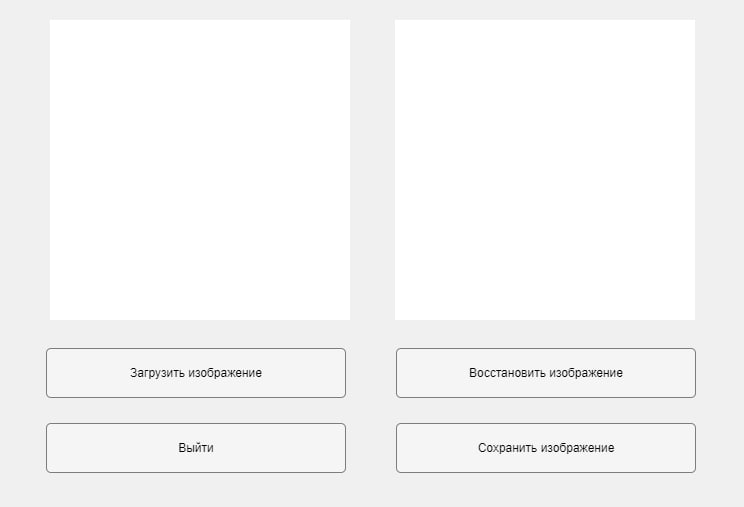
\includegraphics[scale=0.75]{assets/gui}
	\caption{Пользовательский интерфейс программного обеспечения}
	\label{gui}
\end{figure}

Разработанный интерфейс позволяет выбрать исходное цифровое изображение для обработки из файловой системы, применить операцию восстановления к загруженному изображению, а также сохранить полученный результат в отдельный файл.

Процесс выполнения операции восстановления может превышать комфортное время реакции интерактивной системы для человека, в связи с чем при обработке выводится специальное уведомление (рисунок \ref{wait}).

\begin{figure}[H]
	\centering
	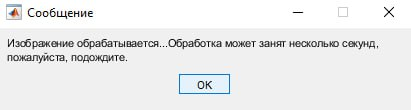
\includegraphics[scale=1]{assets/wait_msg}
	\caption{Уведомление о возможном превышении времени реакции системы}
	\label{wait}
\end{figure}

При попытке восстановить изображение без предварительной загрузки исходного изображения также выводится специальное уведомление для пользователя (рисунок \ref{load}).

\begin{figure}[H]
	\centering
	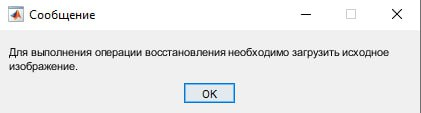
\includegraphics[scale=1]{assets/load_msg}
	\caption{Уведомление о необходимости предварительной загрузки изображения}
	\label{load}
\end{figure}

\section{Сборка и запуск проекта}

В случае, если на персональный компьютер пользователя уже установлен MatLAB, то для сборки и запуска разработанного ПО необходимо выполнить следующие шаги:

\begin{itemize}
	\item проверить наличие компонентов Image Processing Toolbox и Signal Processing Toolbox; 
	\item проверить, что все необходимые файлы и функции, связанные с проектом, находятся в одной папке или в структурированной иерархии папок;
	\item запустить программу MatLAB на компьютере;
	\item открыть папку проекта;
	\item запустить ПО либо через консольный интерфейс (gui.m), либо через соответствующую кнопку <<Run>> в панели инструментов.
\end{itemize}

В случае, если MatLAB не установлен, то необходимо выполнить следующие шаги:

\begin{itemize}
	\item проверить, что исполняемый файл и другие файлы, связанные с проектом, находятся на целевой машине пользователя;
	\item запустить исполняемый файл;
	\item пройти инсталляцию компонента MatLab Runtime~\cite{runtime}, предлагаемую при первом запуске проекта, с целью загрузки минимально необходимого программного обеспечения для запуска проекта без лицензионного экземпляра Matlab; 
	\item запустить проект.
\end{itemize}